\subsection{Comparing Integer Linear Programing to Meta-heuristics}

In this section, we are going to compare the execution results of the Cplex ILP solver and the two metaheuristics algorithms. We are going to solve the problem instances of the medium size data set with our three solvers and plot the results in terms of solving time and objective function. All executions have been performed on the same computer. The parameters for the BRGKA and GRASP algorithms are respectively kept with the same values during all executions. For this experiment, the size of the problems will be determined by the time it takes the ILP solver to find the optimal solution.\\


\begin{figure}[h!]

\begin{subfigure}[b]{.49\linewidth}
\centering
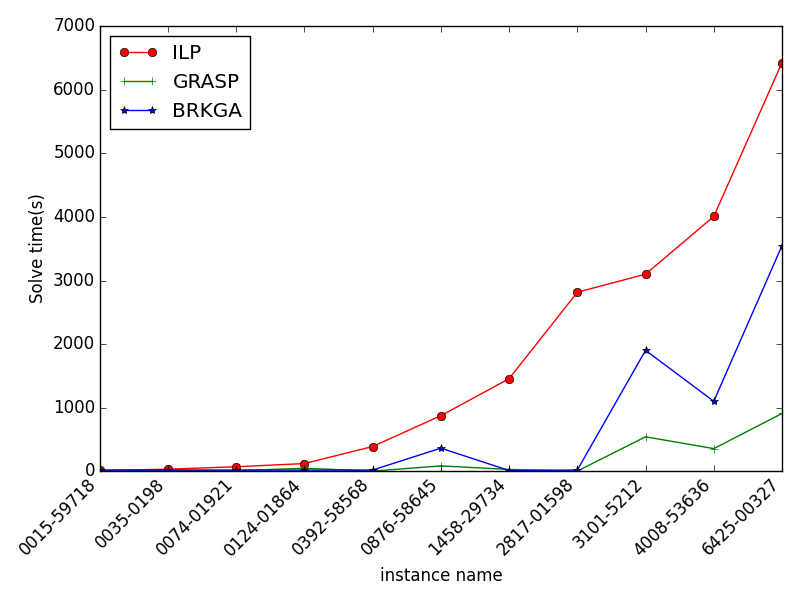
\includegraphics[width=\linewidth]{./img/ILPvsMetah_times.png}
\caption{ Solving times for 38 instances of the mediume set}\label{fig1a}
\end{subfigure}%
\begin{subfigure}[b]{.49\linewidth}
\centering
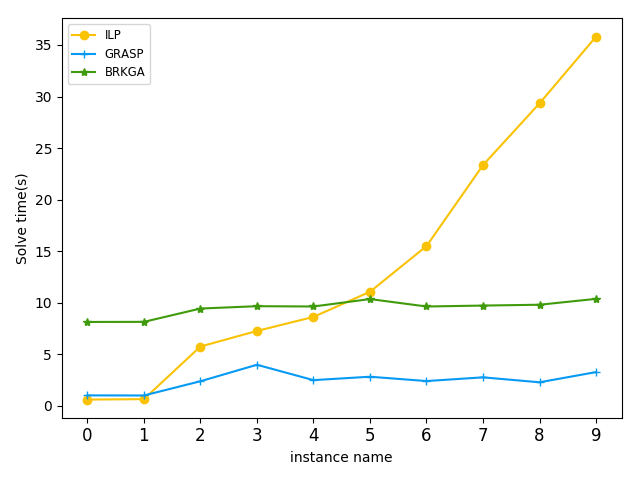
\includegraphics[width=\linewidth]{./img/ILPvsMetah_times_first10.png}
\caption{ Solving times for the first 10 instances }\label{fig1b}
\end{subfigure}\vfill
\begin{subfigure}[b]{.49\linewidth}
\centering

\includegraphics[width=\linewidth]{./img/ILPvsMetah_objf_hist.png}
\caption{Objective function values for 38 instances of the medium set }\label{fig1c}
\end{subfigure}
\begin{subfigure}[b]{.49\linewidth}
\centering
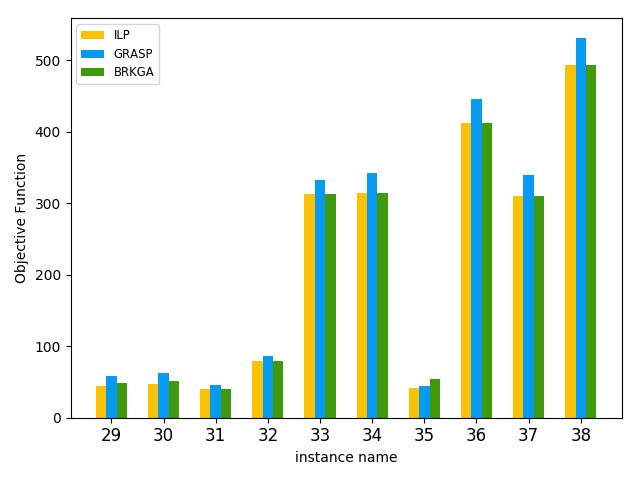
\includegraphics[width=\linewidth]{./img/ILPvsMetah_objf_hist_last10.png}
\caption{Objective function values for the last 10 instances  }\label{fig1d}
\end{subfigure}
\caption{Solving times in seconds (\subref{fig1a}, \subref{fig1b}) and objective function values (\subref{fig1c}, \subref{fig1d}) for the instances of the medium size set solved by ILP, GRASP and BRKGA.  }
\label{fig_ilp_vs_meta}
\end{figure}


The figure~\ref{fig_ilp_vs_meta} on page~\pageref{fig_ilp_vs_meta}, shows that the ILP execution times increase exponentially as the size of the problem instance increases, whereas the GRASP and BRKGA solving times increase much more slowly.
We observe that for the bigger instances, the GRASP algorithm produces worse results (bigger objective function values), whereas the BRKGA produces results very close to the optimum objective function found by the ILP solver.

\pagebreak